\chapter{Relativistic Hartree-Bogoliubov Theory}

From a relativistic energy density functional


DIRHBS for spherical code (DIRHBZ for axially deformed calculations. DIRHBT for triaxial deformations, octupole and tetrahedral calculations)
Today we only focus on this one. 

\section{The Aims}
How can we describe the ground state of an atomic nucleus, a self-bound system of up to a few hundred interacting nucleons, with a single theory that also tells us when its numbers are reliable. 

Ground state properties: Binding energy, density distributions, separation energies. 

The aim is to understand how a relativistic energy density functional describes nuclei. We will see how pairing correlations are added, which are needed for open shell nuclei (in which the shells are not fully occupied. Take \ce{^{132}Sn} is a double magic nucleus, we don't have any pairing correlations) and how the RHB equations follow. 

Roadmap: Many-body problems (nuclei, forces) then mean field (independent particles, EDFs) then relativistic mean field (Dirac, mesons) then add mean field pairing intereaction for open shell (pairs, quasiparticles) then combine everythign in the RHB equations then finally DIRHBS from equations we get numbers. 


\section{Force Between Nucleons}
Short upto a few fm. Pion tail is weak beyond 2fm. Protons also feel Coulomb repulsion. Consequence: There is no simple exact formula, we will need an effective description, fitted to nuclei. 

\section{Many-body Problem}
We want to describe the nucleus using a microscopic model, but it is difficult. For the full quantum state, the wavefunction, \(\Psi\) describes the simultaneous positions of all nucleons, it has \(3A\) spatial coordinates for a nucleus of \(A\) nucleons. The other problem is that nucleons are fermions, when two fermions are switched, the sign of the wavefunction changes. And when nucleons move slightly, their interaction changes the motion. Altogether, the general many body description has joint amplitudes for all configurations, \(\Psi(x_1,x_2,...,x_A)\).

So, we simplify this by restricting the state - let the nucleons move in a common potential and have single particle orbitals in a self-consistent field combined into one antisymmetric state. We describe these states using the Slater determinant. 

\section{Nucleons Behave as Independent Particles}
The experimental evidence for nucleons behaving as indep particles is the existence of magic numbers. This is explained if each nucleon occupies its own level in a common potential, like electrons in an atom. Large gaps give the magic numbers. A plain potential gives 2, 8, 20, 40, 70. Spin-orbit coupling is needed to give the correct magic numbers.

\section{The Mean Field Idea}
Every nucleon interacts with every other. Its complex. So instead we say each nucleon moves independently in an average potential, \(U\). So in the schrodinger eqn we have the common potential, and the s-o coupling term (for the magic gaps). Solving this equation gives the single particle functions.

\section{Filling the Levels gives the density}
Each level j holds \(2j+1\) protons and \(2j+1\) neutrons. All nuclei have nearly the same interior density, around \(0.15\)fm\(^{-3}\) i.e. nuclear matter saturates. Only the radius grows with the number of nucleons. Only \(s\) orbitals reach \(r=0\), hence the \ce{^{40}Ca} peak.

\section{The Nucleons Make their Own Potential}
We start to form \(U(r)\) by making a guess e.g. the Woods-Saxon well. 

Then we solve for orbitals (mean field. The nucleons create \(U\) from their own density).

Then we look for the densities, calculated from the wavefunctions from step 2 and the occupation probabilities of the levels.

Then from the densities, we calculate the new density-dependent potential from the new functional. When the U converges, we stop iterating. 

If you start the loop from different guesses of U, any reasonable guess reaches the same point. However, if you are dealing with deformed nuclei, you may end up in a local minimum. Today, we only look at spherical. 

\section{The Potential From an Energy Density Functional}
Remember the three main models: ab initio (try and solve eqns explicitly by including everything), shell model and DFT. For ab initio, we can't do the whole nuclear chart - only up to \(A=16\). For shell model, there are also computational limits. One of the most important advantages of DFT is that we don't have limits - we can look at the whole nuclear chart, but we don't know if our answer is correct, since we don't know the exact Hamiltonian, its an approximation. 

We write an energy density functional, \(E[\rho]\). The potential is how much the energy changes when a little density is added at \(r\).
\[U(r) = \frac{\delta E}{\delta \rho (r)}\]

\section{Families of Nuclear Energy Density Functionals}
Split into two parts, non-relativistic (Skyrme and Gogny) and relativistic. All three of them reproduce the masses they were fitted to, but their predictions will differ the most for neutron-rich nuclei and along the driplines (we have experimental data along the stability line but not much around the driplines). We have a functional, optimise it using nuclei around the stability line - this embeds the info from these nuclei, not the ones near the driplines. 

\section{Why a Relativistic Description?}
Its not because the nucleons are fast. At the Fermi surface, \(v\approx 0.3c\). Its moret o do with the strucre of the model. Comparing the relativisitc to the non-relativsitic makes it clear. Take a non-relativisitc like Shyrme, the spin-orbit is an additional term. In the relativistic, its integral in the description. Relativisitc functionals also describe saturation and exotic nuclei very well. Also, for rotating nuclei and odd nuclei (time odd fields) follow from Lorentz covariance, no new parameters.


\section{From Schrodinger to Dirac}
 

From the Lagrangian, in the relativistic framework, the scalar potential is \(S \approx -400\) MeV and the vector potential is \(+350\) MeV for the strong interaction. These two things come from exchanging mesons. Both are enormous, so why is a nucleon bound by only about \(8\) MeV? The orbital feels the summation, \(-70\) MeV. 

meson exchange vs point coupling have lagrangians constructed differently. 


Task 1: Benchmark \ce{^{132}Sn}

\begin{figure}
    \centering
    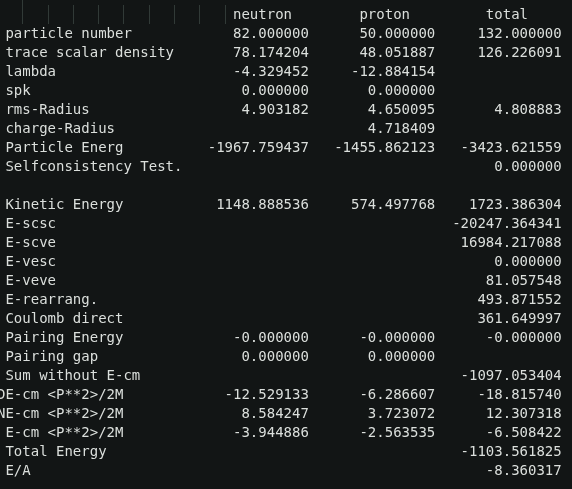
\includegraphics[width=0.8\textwidth]{assets/2.1.8_fortran_132Sn.png}
\end{figure}


Task 2: Is the Basis Large Enough? \ce{^{120}Sn}
Columns two to six come from the output file. \(E\) is \code{Total Energy}
\begin{tabular}{cccccc}
  \toprule
  $N_F$ & $E$ (MeV) & $r_{\mathrm{ch}}$ (fm) & $\Delta_n$ (MeV) & $\lambda_n$ (MeV) & $E(N_F) - E(N_F - 2)$ \\
  \midrule
  10 & 1020.467115 & 4.639769 & 1.214296 & 7.607345 & \(-\)\\
  12 & 1019.399061 & 4.644893 & 1.317889 & 7.725233 & -1.068054\\
  14 & 1019.341640 & 4.647371 & 1.328869 & 7.743290 & -0.057421\\
  16 & 1019.428493 & 4.646582 & 1.326419 & 7.725996 & \(+\)0.086853\\
  18 & 1019.310616 & 4.646698 & 1.327245 & 7.721293 & -0.117877\\
  20 & 1019.222751 & 4.647186 & 1.326870 & 7.723283 & -0.087865\\
  \bottomrule
\end{tabular}